\section{Grundlagen}\label{kap:grundlagen}
In diesem Kapitel werden einige Grundlagen für die in Kapitel \ref{kap:featureextraktion} diskutierten Algorithmen besprochen.
\subsection{Was sind Sensordaten}\label{kap:sensordaten}

Um den Ablauf einer Maschine zu koordinieren und den aktuellen Zustand zu Überwachen werden oft Sensoren an den Maschinen angebracht. 
Diese Daten werden zu definierten Taktzeiten aufgenommen und weiterverarbeitet. 
Es kann sich dabei um einfache Kontaktsensoren handeln, mit einer begrenzten Anzahl an Zuständen oder Sensoren mit einem reellen Zustandsbereich wie Umgebungssensoren (Luftdruck-, Temperatursensor, etc.). 
In Abbildung\ \ref{fig:datasetoffice} sind Sensordaten in Form eines Datenplots dargestellt. 
Es handelt sich um Licht-, Temperatur- und Drucksensordarten aus einem Büro im Zeitraum eines Arbeitstages. 
Abgebildet sind die Sensordaten zwischen $6:00$ Uhr und $19:00$Uhr.
\begin{figure}
    \centering
    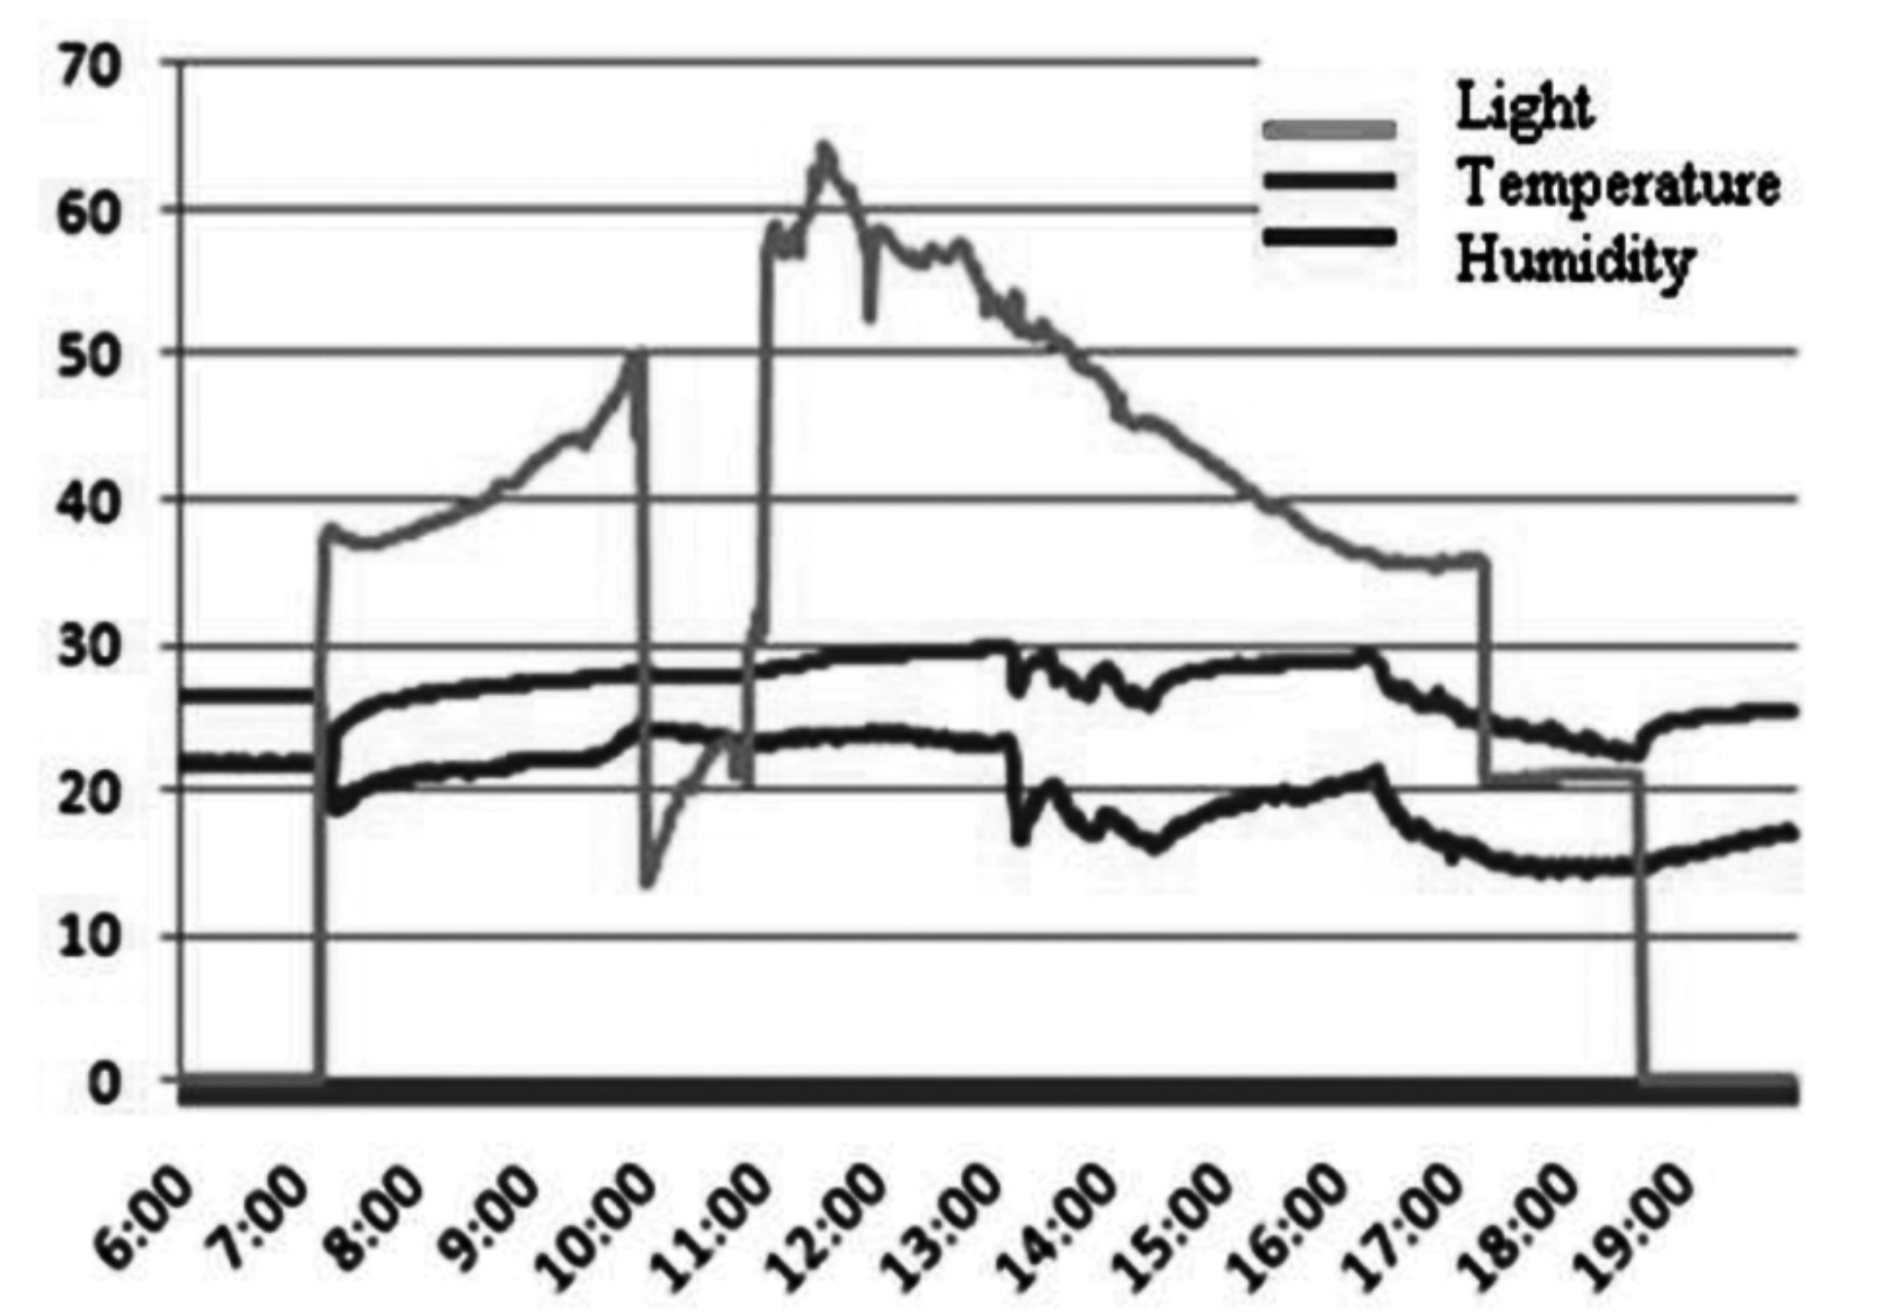
\includegraphics[width=.8\textwidth]{datasetOffice.png}
    \caption{Sensordatenabweichung anhand von Licht, Temperatur und Luftfeuchtigkeit im Buro innerhalb von einem Arbeitstag~\cite{moraru2010using}}
    \label{fig:datasetoffice}
\end{figure}

Um solche Sensordaten mathematisch weiterverarbeiten zu können, werden sie in Vektorform gebracht.
Ein Datensatz zum Zeitpunkt $6:00$ Uhr mit den Werten Licht = $0$, Temperatur=$22$ und Luftfeuchtigkeit = $25$ könnte dargestellt werden als:
\begin{equation}
    x_1 =
  \begin{pmatrix}
      0\\
      22\\
      25
  \end{pmatrix}
\end{equation}

Ein Vektor enthält somit einen Seonsordatensatz zu einem Zeitpunkt. Um Zeiträume darzustellen werden die Daten in eine Matrixform gebracht. Beispielsweise erhält man bei einer Stündlichen Abtastrate und einem Zeitraum von $8:00$ Uhr bis $17:00$Uhr folgende Matrix:
\begin{equation}
    x_{1,10}
    \begin{pmatrix}
       38 & 40 & 46 & 24 & 60 & 58 & 51 & 44 & 40 & 36\\
       20 & 22 & 22 & 24 & 24 & 24 & 20 & 18 & 20 & 17\\
       25 & 28 & 28 & 28 & 29 & 30 & 20 & 27 & 29 & 26
    \end{pmatrix}
\end{equation}

Diese mathematische darstellung ist nur ein Beispiel und kann beliebig strukturiert werden.

Die erzeugte Matrix kann anschließend als Eingabe für Analysealgorithmen dienen.
Schon bei diesen geringen Datenmengen entsteht eine $K x N $ große Matrix, wobei $K=$ Anzahl der Paramter (Sensoren) und $N=$ Anzahl der Daten.

Sollen auch noch Daten Raumübergreifend analysiert werden, können diese in Form eines Tensors dargestellt werden. Bei $M$ vielen Räumen entsteht ein $K x N x M$ großer Tensor.
Schon anhand dieses simplen Beispiels wird die Datenmenge und Komplexität der Daten ersichtlich.
In der Maschinenüberwachung entstehen dadurch schnell Datensätze im Millionenbereichen und da jede Komponente einer Maschine oft mit mehereren Sensoren ausgestattet ist, entstehen riesige Tensoren.

Neben klassischen Regressionsverfahren zur Datenanalyse, welche oft für Anomliedetektionen verwendet werden, gibt es auch verschiedene Klassifikationsverfahren. Dazu werden den Datensätzen manuell oder automatisiert Klassen hinzugefügt.

Mathematisch dargestellt erhalten wir dann einen Datensatz zum Zeitpunkt $t_1$ in Form eines Tupels $\tau_1=(t_1,x_1)$. Diesem Tupel wird abhängig von den verwendeten Verfahren eine Klasse $y_1$ zugewiesen~\cite{gay2013feature}. Für den Zeitraum $(t_1,...,t_n)$ mit $n \in \mathbb{N}$ vielen Daten erhalten wir den Datensatz 
\begin{equation}
  D=\{ (\tau_1,y_1), ... , (\tau_n,y_n) \}
  \label{equ:trainingset}
\end{equation}
Das Ziel kann es sein das Tupel $(t_{n+1},y_{n+1})$ voherzusagen.

Es werden auch nicht nur feste Zeiträume betrachtet. 
Durch dauerhaft laufende Maschinen entstehen kontinuierliche Datenströme.
Daraus folgt ein kontiniuerlich wachsender Datenbestand.
Um ressourcenschonend und möglichst in Echtzeit die Daten zu analysieren, werden harte Speicher- und Laufzeitbedinungen an Analysealgorithmen gestellt.


\subsection{Feature Extraktion}\label{kap:featureextraktionuebersicht}
In Kapitel \ref{kap:sensordaten} wurde ein Datensatz durch seine Muster und Merkmale beschrieben. Merkmale können einfache Parameter, wie Schwellwertüberschreitungen sein. In Komplexeren Datenstrukturen, können die Daten anhand von Verlaufsmustern unterschieden werden. 

Um Algorithmen zu trainieren die Daten durch diese Merkmale und Muster zu unterscheiden, gibt es zwei wesentliche herangehensweisen. Es können die Merkmale dem Algorithmus vorgegeben und auf diese Merkmale trainiert werden, oder es werden Verfahren angewendet um diese Merkmale zu extrahieren. Es ist die Rede von \enquote{Feature Extraktion}. Ein \enquote{Feature} ist eines dieser Merkmale, wodurch Daten in einem Datensatz voneinander unterschieden werden können. 

Dabei ist das Ziel die Features so zu wählen und zu parametrisieren, dass das der ermittelte Wert dem tatsächlichen Wert möglichst ähnelt. Betrachten wir die Gleichen \ref{equ:trainingset} und die daraus ermittelte Funktion $p(x_i)$, welche das Ergebnis des gewählten Algorithmus und des Trainingsdatensatzes ist. Es soll versucht werden den Fehlerunterschied

\begin{equation}
  \sigma = p(x_i)-y_i
\end{equation}

möglichst zu reduzieren~\cite{gensler2015fast}. Konkret wird meist die Summe der Quadratischefehler
\begin{equation}
  \sigma^2 = \frac{1}{N} \sum_{i=0}^{K}(p(x_i)-y_i)^2
\end{equation}
versucht zu reduzieren.

\begin{center}
  - TODO - Ein konkretes Beispiel für Feature Extraktion raussuchen und daran erkären. Es muss auch noch die Notwendigkeit und die herangehensweise von Dimensionsreduzierung erläutert werden.
\end{center}

\begin{itemize}
  \item Kurze ML einleitung mit erklärung zur Feature-Extraktion
  \item Feature extraction vs Feature selection
  \item \enquote{extrahieren von Merkmalen, wodurch die Daten in einem Datensatz voneinander unterschieden werden können}
\end{itemize}